\chapter{相关技术}{Related Technology}
\section{Hadoop技术}{Hadoop Technology}
自从Google公司公布分布式计算三架马车MapReduce、GFS和BigTable之后,Apache基金会开放了
Hadoop大数据计算平台,并发展成为Apache顶级项目,包含了Google公司三架马车的开源实现,分别为
Hadoop MapReduce、HDFS和HBase。Hadoop一经推出备受开源社区广泛关注,其拥有较高的容错性、可靠性和适用性等
优点,最重要的是Hadoop可部署在廉价的普通PC机器上,大大降低开发成本。Hadoop MapReduce是Hadoop的计算
模型,该模型将所有数据处理流程分解为Map阶段和Reduce阶段\cite{Dean2004MapReduce},这个计算模型的优势
在于使用简单,它隐藏了并行化、容错、位置优化和负载均衡的细节,使得没有并行和分布式经验的开发人员能够处理业务逻辑,
这也是Hadoop成为大数据计算框架被广泛关注和研究的原因。

\subsection{HDFS机制}

HDFS是Hadoop分布式计算框架中数据存储基础,同其他分布式文件系统PVFS(Parallel Virtual File System)、
Lustre和GFS一样,HDFS将系统元数据存储在特定的节点上,称之为NameNode;应用程序所需数据存储在其余的节点上,
称之为DataNode。为了保证容错性,需要指定特定节点作为SecondaryNameNode,它是NameNode的备用节点,负责
拉取主控服务器的日志。当NameNode发生失效,替代原来的NameNode的进行工作,所有节点使用TCP协议进行连
接和通信\cite{Shvachko2010The}。

HDFS采用主从结构,集群一般由一个NameNode和多个DataNode组成。不同于PVFS和Lustre的RAID(Redundant Array of 
Independent Disks)文件保护机制,HDFS将数据文件切分成若干数据块(Block),默认为64M,将这些文件分散到不
同DataNode节点并且每个数据块拷贝若干份,通过这些措施来提高数据的可靠性,图\ref{fig:hdfsarchitecture}为HDFS体
系结构。
\begin{figure}
\centering
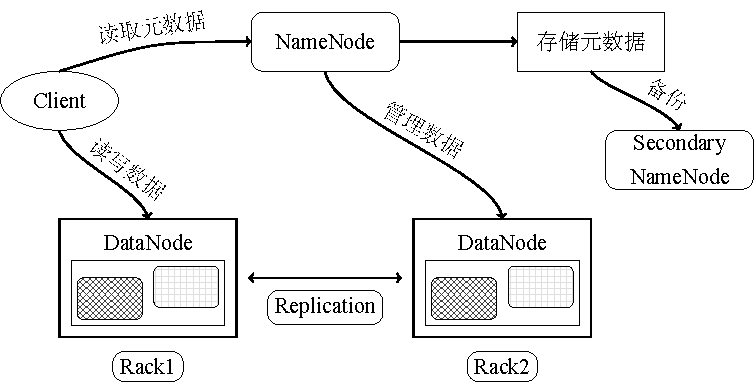
\includegraphics[width=0.9 \linewidth]{figures/hdfs.pdf}
\caption{HDFS体系结构}{HDFS architecture}
\label{fig:hdfsarchitecture}
\end{figure}

HDFS对数据的操作主要表现为数据的读写和数据块的备份:

数据读写操作:当客户端(Client)向NameNode发起读取数据请求,NameNode通过元数据判断该数据存在,如果存在,HDFS将返回该
数据所在的详细位置给客户端。客户端将使用TCP协议与数据对应的DataNode进行通信读取数据;数据写入的过程与之稍微不同,
客户端同时向NameNode和DataNode发送请求,当NameNode接收到来自DataNode的消息立即返回确认消息,DataNode开始进行数据
写入。

数据块备份操作:对于较大的集群,由于DataNode众多,不可能同时管理Block。通常将将这些Block分布在不同的机架上,
机架内部通信带宽往往比机架间大得多。因此通过NameNode接受来自DataNode的心跳和Block的报告,将Block备份到不同
的节点和机架上\cite{Oriani2012From}。

\subsection{MapReduce编程模型}

Hadoop MapReduce是Google MapReduce开源实现,其核心思想则是源于函数式编程语言。它将分布式业务逻辑从
复杂的细节中抽象出来,开发人员只需要关注Map函数和Reduce函数便可以通过集群系统来执行程序,实现分布式计算,而
无需关注消息传递和计算任务分配等复杂的问题。

Map阶段关注的是任务的分解,通过Map算子将每个输入输出组成Key/Value键值对作为输入和输出形式。Reduce算子是
对Map算子的输出进行汇总,以Key按照特定的分区算法,并行执行Reduce函数。

以Word Count任务为例,MapReduce运行机制见图\ref{fig:mapreduce},按照执顺序包括:输入分片(Input Split)、Map阶段、Shuffle阶
段和Reduce阶段\cite{SinghMapReduce}。
\begin{figure}
    \centering
    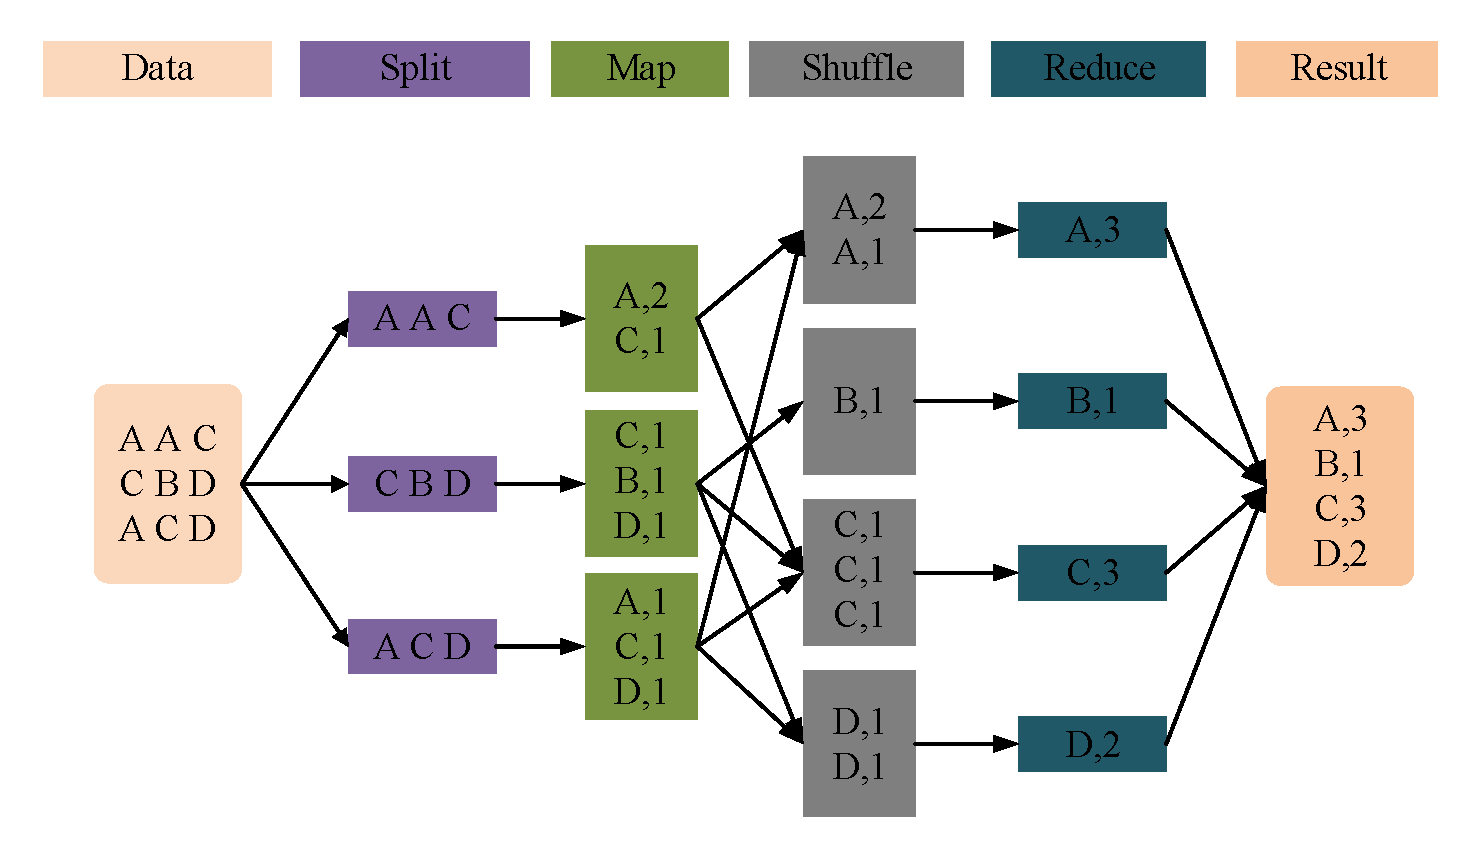
\includegraphics[width=0.8 \linewidth]{figures/mapreduce.pdf} \\
    \caption{Word-Count处理流程}{Word-Count procession}
    \label{fig:mapreduce}
\end{figure}

(1)输入分片:在进行Map计算之前,MapReduce会根据输入数据计算输入分片,每个输入对应着一个Map任务,输入分片和HDFS
数据文件的Block相关,即每个输入数据文件是HDFS默认大小的整数倍,不满整数向上取整。如果存在较多的小文件,将会
导致Map执行阶负载不均衡。

(2)Map阶段:开发人员重写Map函数,以满足特定的业务逻辑需求,而且Map函数一般在数据所在节点执行,从而降低了通信消耗时间。

(3)Shuffle阶段:Map阶段到Reduce阶段之间过程就是Shuffle过程,也是MapReduce性能提升的重点地方。MapReduce计算
的是海量数据,内存中不可能存储所有数据,Map阶段在输出时会将部分数据写入磁盘,等Map输出所有数据后,Map会采用
类似归并排序(Merge Sort)算法对输出结果合并。这个过程中会有一个Partitioner操作。每个Partitioner操作对应
一个Reduce作业,Partitioner就是Reduce阶段输入分片,开发人员可以编写Partitioner函数,提高Reduce阶段执行效率。

(4)Reduce阶段:对来自Shuffle阶段的输入数据进行汇总处理,开发人员根据业务需求,自行编写Reduce函数,并将结果数据
存储在HDFS上。
\subsection{MapReduce不足}
在Hadoop$1.0$版本中,MapReduce框架有唯一的Master、JobTracker和每个集群节点一个Slaver、TaskTracker共同组
成。其缺点显而易见,JobTracker是MapReduce的集中处理节点,存在单点故障的风险;JobTracker完成了太多的任务,造
成了过多的资源消耗等。在Hadoop$2.0$版本中,推出了YARN(Yet Another Resource Negotiator)统一的资源管理平台,该
平台能够很好地将不同的任务隔离开来,增加集群的健壮性。

虽然MapReduce通过高度抽象,能够很好地描述大部分业务逻辑,但还是过于底层。简单的过滤(Filter),分组(Group by)等
操作都需要编写冗长的Map和Reduce接口函数,无形中增加了开发人员的负担和出现故障的概率\cite{Grolinger2014Challenges}。
而且整个流程中的中间过程数据都要缓冲到HDFS中,磁盘IO时间开销都是系统性能的瓶颈,尤其是针对数据挖掘、机器学习等需要
反复迭代的算法,MapReduce编程模型往往是捉襟见肘。

\section{Spark计算框架}{Spark Framework}
Spark作为炙手可热开源并行计算框架,吸收和借鉴了MapReduce思想,并提出了新型的内存计算模型,将整个计算过程中数据保存在
集群内存中,从而大大提高了Spark表现力。Spark同样隐藏了并行化的细节,使用者只需要关心业务需求。
\subsection{Spark框架体系}
BDAS(the Berkeley Data Analysis Stack)是AMP实验室打造的一个开源的大数据处理一体化的技术生态系统,见图\ref{fig:sparkarchitecture},
整个生态主要分为三大部分,核心部分为Spark Runtime支持的Spark Core,其包含了Spark最基本、最核心的功能和基本分布式并行
计算算子,这些算子提供了Java,Scala,Python和R编程语言接口。在上层部分是为处理特定业务场景而设计的生态组件,是Spark的高层组件,
分别为:结构化查询工具Spark SQL、分布式机器学习库MLlib、并行图计算框架GraphX和流计算框架Spark Streaming。
底层为集群管理器,如YARN,Mesos等等,保证了Spark运行框架运行的健壮性。
\begin{figure}
\centering
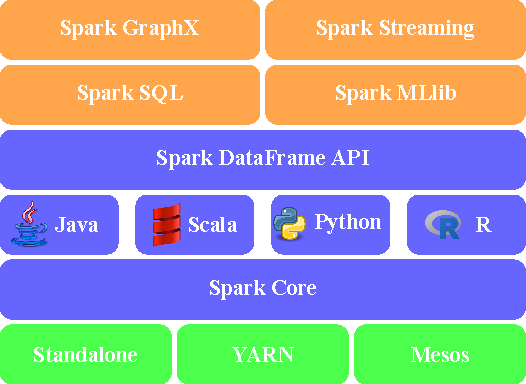
\includegraphics[width=0.6 \linewidth]{figures/spark.pdf} \\
\caption{Spark体系架构}{Spark architecture}
\label{fig:sparkarchitecture}
\end{figure}

(1)Spark SQL

Spark SQL是Spark $1.0.0$ 版本中新加入的组件,是Spark生态系统中最活跃的组件之一,为结构化数据提供了方便的存储和查询
操作\cite{Guller2015Spark}。Spark SQL提供了方便的调用接口,用户可以通过使用Scala、Java、Python等开发基于Spark SQL API的数据处理
程序,也支持传统的SQL语句与Spark进行交互。

(2)Spark MLlib

Spark MLlib(Spark Machine Learning library)常用的机器学习算法的实现\cite{MllibMLlib}。
Spark MLlib的在机器学习方面优点主要有以下三点:\circled{1}Spark是内存计算的计算框架,这一点非常适
合机器学习算法迭代计算的特点,避免Hadoop MapReduce这类IO频繁的计算框架;\circled{2}Spark MLlib使
用和部署非常方便,支持Scala和Python交互式开发环境,方便机器学习算法使用人员快速验证算法原型系统;\circled{3}Spark MLlib作
为Spark生态系统的子成员,可以去Spark生态系统进行无缝结合。

(3)Spark GraphX

是Spark分布式图计算框架,它是常用图算法在Spark上的并行实现,并且提供了图计算中用于图和图计算中的API。
是Graph Lab和Pregel在Spark上的重写及优化,是Spark生态圈中非常重要的组件\cite{Xin2013GraphX}。

Spark GraphX的核心抽象概念是弹性分布式属性图(Resilient Distributed Property Graph),是一种点和边都带有属
性的有向多重图。它扩展了Spark RDD的抽象,实现了统一表示。弹性分布式属性图有Table和Graph两种视图,对应的这两种
视图只需要一份物理存储,两种视图都有各自的操作符,基于Spark的RDD可以很轻松的进行操作。通过分布式计算提高了效率。

(4)Spark Streaming

Spark Streaming是建立在Spark上流应用计算框架\cite{Guller2015Sparks},它将流式计算分解成一系列短小的批处理作业,也就是将输入数据
按一定大小划分为一段段的数据(Discretized Stream),每一段数据都RDD,然后将Spark Streaming中
对DStream的Transformation操作变为针对RDD的Transformation操作,将RDD经过操作变成中间结果保存在内存中。
\subsection{RDD介绍}
弹性分布式数据集RDD,是Spark的核心抽象,是对分布式内存的抽象表达,它表示已被分区、只读的、并提供了一组丰富的操作方式
来操作这些数据集合。这些数据集可以全部或者部分缓存在内存中,在多次计算间重复使用,省去了大量的磁盘IO操作。

现有的并行计算框架的数据结构在处理两种应用场景显得不够高效:\circled{1}迭代式计算,主要为分布在图计算领域和机器学习问题中;\circled{2}
交互式计算工具,操作能够立即返回结果。RDD通过高度受限的共享内存方式解决上述问题,
基于稳定物理内存中的数据集合执行批量操作(如Map,Join和Group by)
操作。与其他分布式共享内存系统选择检查点(Check Points)和回滚(Roll Back)机制不同,RDD选择血统(Lineage)机制来保证可靠的容错性,
每一个RDD记录如何从RDD中衍生出来的,一旦某个RDD发生数据丢失,根据这些记录进行重新构建,而不需要进行高昂代价的检查点操作来进行数据恢复。
虽然RDD不是通用的共享内存的抽象,却包含了高可靠性、强可伸缩性和良好的表述的能力,因此成为了Spark一切操作的核心。

RDD从本质上来讲,就是只读的集合,不过集合是分布在不同的分区上的,每个分区就是一个Dataset。RDD在进行转换的过程中产生了依赖,
如果RDD的每个分区被一个子RDD继承,那么称之为窄依赖(Narrow Dependency);若RDD的分区被多个子RDD继承,那么称之为宽依赖(Wide Dependency)。
不同的操作产生不同的依赖。图\ref{fig:dependency}分别展示了map产生的窄依赖和join产生的宽依赖\cite{Zaharia2012Resilient}。
\begin{figure}
\centering
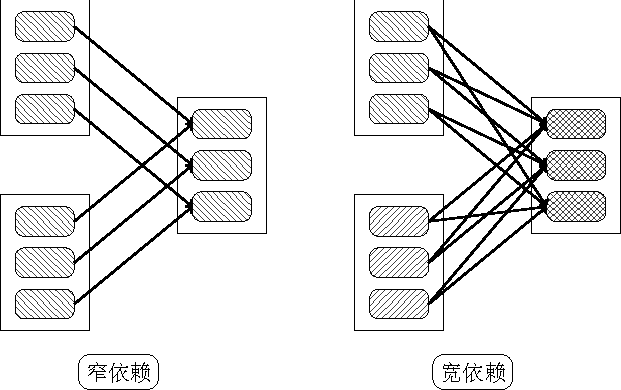
\includegraphics[width=0.6 \linewidth]{figures/rdd.pdf} \\
\caption{窄依赖和宽依赖}{Narrow dependency and wide dependency}
\label{fig:dependency}
\end{figure}

RDD提供了丰富的编程接口来操作数据集合,主要分为两种:Transformation和Action。

Transformations返回值还是一个RDD,如Map,Filter,Union等操作。它可以理解为任务分配的过程,其采用的是Lazy策略,如果是
只提交Transformation是不会提交任务执行,只有在Action操作的时候才回被触发。

Action操作是将RDD持久化起来,每调用Action操作,都会触发一次Spark的作业提交,将规划的任务(Job)提交给计算引擎,由计算
引擎将其分为多个Task,再分发相应的计算节点,开始真正处理过程。从目前的Spark的API来看,Action操作主要分为两种:\circled{1}Action操作
将标量或者集合返回给Spark的客户端程序。\circled{2}Action操作将RDD直接保存到外部文件系统或者数据库中。
\subsection{Spark优势}
Spark一栈式解决方案有很多优势,具体如下:

(1)快速处理。由于Spark采用内存计算,避免了Hadoop的磁盘操作,节省了I/O操作,在迭代式计算上Spark有着明显的优势。

(2)通用性强。Spark提供了一个强大的技术堆栈,是一个可以处理流式处理、机器学习、即时查询、图分析等多种无缝大数据处理链接计算平台。

(3)可以与Hadoop集群集成。Spark可以单独运行,也可以运行在Mesos、Yarn等集群资源管理系统上,也可以读取已有的任何HDFS数据。
\section{空间数据挖掘}{Spatial Data Mining}
空间数据挖掘是多门学科交叉研究领域,包含了多种研究技术,常用的方法有但不仅限于地理信息系统、计算几何、模式识别、机器学习、深度学习等。因此
空间数据挖掘技术丰富多彩,下面简单介绍几种常用的方法。

(1)统计分析方法 

统计方法是空间数据分析最基础的方法,以数学统计知识为基础。关注点是空间对象的非空间属性,简单的统计方法有最大值,最小值,平均值,方差等等,
复杂的方法有方差分析,P值估计等等,通常来讲这些统计结果都用图表进行表达。

(2)聚类分析方法

聚类分析方法是非监督数据挖掘中最主要的方法,通过对空间对象相似性判断,将整个空间对象划分为若干簇\cite{杨春成2004空间数据挖掘中聚类分析算法的研究}。
在聚类算法中,距离函数非常重要,常见的距离函数选择有欧几里得距离、曼哈顿距离和更通用的$L_p$距离,除了数值型属性之外,空间聚类还需要将空间位置纳入
考虑范畴,因此不同属性的应当赋予不同的权重。

(3)空间分析方法

空间分析是空间数据挖掘的特色,通过各种空间分析,对空间信息进行加工,从而发现更多知识。常见的方法有空间缓冲区分析、空间
核密度分析和空间趋势面分析等等,空间分析常常结合地学第一定律进行统计分析,拓展了统计分析方法关注的内容,发现新的知识\cite{李小文2007地理学第一定律与时空邻近度的提出}。

(4)空间关联规则挖掘方法

关联规则挖掘是根据销售事务数据库交易项商品同时出现的规律\cite{曾玲2005关联规则在空间数据挖掘中的研究},Apriori算法是关联规则挖掘最著名的
算法。空间关联规则是关联规则在空间方面的拓展,将空间关系纳入到考虑范畴。以空间关联为基础,发展出空间同位模式挖掘,比如生物在生态环境
中的共生现象。

\section{新浪微博数据接口}{Weibo API}
目前新浪微博数据获取方式主要有两种:\cite{廉捷2011新浪微博数据挖掘方案}:\circled{1}通过网络爬虫程序获取数据;
\circled{2}通过新浪微博提供了API接口获取相应主题的数据。

网络爬虫是能够自动获取并下载网页的计算机应用程序\cite{Nemeslaki2011Web},根据一定
规则不停的向网络服务器发送请求,获取特定的信息。由于互联网是通过URL进行连接,可以不间断
对整个网络内容进行获取,需要制定相应的爬虫策略,一般有与深度优先和广度优先两种调度策略。
互联网服务器则将网页中的文本内容、图片、音频视频等内容发送给应用程序,应用程序则将这些
数据按照特定的格式保存下来。

由于个人用户频繁使用爬虫从网站中获取数据将会对网站服务器带来较大的负载,因此新浪微博之类的网站会从
爬虫程序的IP地址或者验证码方式限制请求次数。而且通过爬虫获取的数据噪声较大,需要进行大量的清洗工作,
因此本文将使用新浪微博API接口获取海量空间数据。
\subsection{微博API使用}
作为丰富数据资源的平台,新浪微博给其他应用程序开放了访问这些数据的API,应用程序通过这些API获取微博内容、用户个人信息、
签到和空间位置等相关信息。这些API其实就是一系列HTTP Get请求,API接口的参数作为请求的参数发送给新浪微博服务器,
新浪微博返回相应的结果。新浪微博将这些API封装到不同编程语言的SDK中,包括了Python、Java,C\#、PHP等。

微博API的使用需要对用户的身份进行鉴别,目前新浪微博对开放平台用户采用OAuth$2.0$的方式进行授权\cite{Recordon2011The}。
OAuth$2.0$授权验证具有简单、安全等特点,是社交网络平台对外开放权限的主要方式,使用流程见图\ref{fig:api}。
\begin{figure}
  \centering
  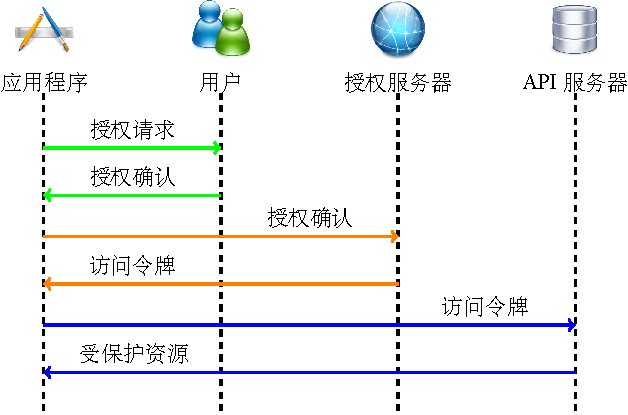
\includegraphics[width=0.6 \linewidth]{figures/api.pdf}
  \caption{新浪微博API使用流程}{The usage of weibo's api}
  \label{fig:api}
\end{figure}

第三方应用程序想要获得API接口的使用权,首先要在新浪微博开发平台进行申请应用程序的AppKey和AppSecret,
这个AppKey和AppSecret是该应用程序的标识码。用户在使用该应用程序的时候,首先要在授权页面登录自己
新浪微博账号,给予授权。然后应用程序将该用户的授权发送给新浪微博的授权服务器,返回访问令牌(Access Token)。
那么该应用可以以访问令牌访问这些API接口,获得相应的数据,在整个获取数据过程中用户的隐私得到保护。


\subsection{空间数据相关API}
新浪微博API接口主要有粉丝服务接口、微博接口、收藏接口、公共服务接口、位置服务接口、
地理信息系统接口和地图引擎接口等,部分空间数据相关API接口说明见下表\ref{tab:weiboapi}。
 \begin{table}
  \centering
  \caption{微博接口描述(部分)}{Description of Weibo api(partly)}
  \label{tab:weiboapi}
  \tabulinesep=1.5mm
  \begin{tabu}to 0.90\linewidth{X[1.1,l, m]X[1.2,l,m]}
    \tabucline[0.1em]-
    \rowfont[c]{} 接口API地址 & 说明 \\
    \tabucline-
    location/geo/address\_to\_geo & 根据地址返回地理信息坐标 \\
    location/pois/search/by\_area & 根据区域按坐标点获取POI点的信息 \\
    location/pois/show\_batch & 批量获取POI点的信息 \\
    location/citycode & 城市代码对应表 \\
    place/nearby/pois & 获取附近的POI点 \\
    place/pois/show & 获取地点的详细信息 \\
    \tabucline[0.1em]-
   \end{tabu}
\end{table}

新浪微博API接口使用非常简单,传入相应的接口指定的参数,即可返回查询结果。
以location/geo/address\_to\_geo接口为例,参数见表\ref{tab:apiparameters}。
\begin{table}
  \centering
  \caption{接口参数说明}{Description of api's parameters}
  \label{tab:apiparameters}
  \tabulinesep=1.5mm
  \begin{tabu}to 0.75\linewidth{X[1,c]X[1,c]X[2.4,l]}
    \tabucline[0.1em]-
    \rowfont[c]{} 参数 & 类型 & 说明 \\
    \tabucline-
    access\_token & String & 采用OAuth授权方式必填参数 \\
    address & String & 需要获取的坐标的实际参数 \\
    \tabucline[0.1em]-
   \end{tabu}
\end{table}

当应用程序通过该接口将符合要求的参数传入发送请求后,服务器将结果以JSON的格式将
结果返回至客户端。

\section{本章小结}{Chapter Summary}
本章首先介绍了Hadoop大数据计算框架,分别介绍了Hadoop分布式存储机制HDFS和
分布式计算模型MapReduce,并分析了其中的优缺点;然后介绍了目前流行的并行
计算框架Spark,着重介绍了Spark的核心数据结构RDD和上层应用接口;接着介绍了
常用的空间数据挖掘算法,最后介绍了新浪微博API使用方法和与空间相关数据获取接口。